\documentclass{article}
\usepackage{graphicx}
\usepackage[utf8]{inputenc}
\usepackage[spanish]{babel}
\usepackage{xcolor}
\usepackage{amsmath}
\usepackage{amssymb}
\usepackage{titling}

\setlength{\parindent}{0pt}
\pagecolor{black}
\color{white}
\title{
    % 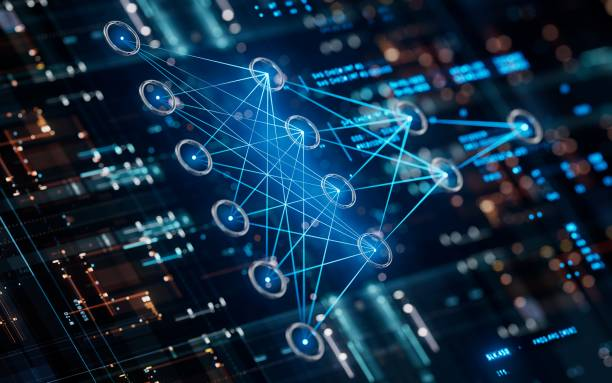
\includegraphics[width=10cm]{imgs/portada.jpg}
    \textbf{Representación y tratamiento de la información}
}
\author{BlasAST}
\date{Junio 2025}

\begin{document}
\maketitle

\newpage

\tableofcontents

\newpage

El objetivo de \textbf{la representación y el tratamiento de la información}
consiste en dotar a los usuarios de la capacidad de identificar principios,
conceptos o recursos elementales sobre los sistemas informáticos, ya sea a
nivel de hardware, software o la representación de datos. Además, se podrá
contrastar los sistemas y técnicas más adecuados para la representación
eficiente de un conjunto de datos.

\newpage

\section{Representación de los Números Enteros sin Signo}
Em nose, aqui lo que se muestra basicamente es porque usamos los
números como los usamos.

\subsection{Introducción a los Sistemas de Numeración}

Bueno, cuando contamos del 0 al 9 podemos darnos cuenta que usamos
solo 10 digitos, el resto de números que usamos estan formados
mediante la combinación de estos números. Esto de que usemos 10 digitos
(simbolos) es lo que se llama sistema de numeración.\\\\¿Qué es un sistema de
enumeración? Pues lo que usamos en nuestro día a día. Es como si en nuestra
cabeza tuvieramos un programa que nos permite diferencia que el 21 y el 12 no
son el mismo número, que expresan distinta cantidad, que ambos estan formados
por el 1 y el 2 pero que influye el orden. Eso es un sistema de numeración.
Un conjunto de simbolos finitos y unas reglas que utilizamos para expresar
distintas cantidades numéricas.\\\\\

La única preocupación que debemos de tener respecto a las restricciones del
sistema son las normas que trae con él, no nos limitan en cuanto a la cantidad
de simbolos ni en la forma en la que podemos usarlos.\\ Tampoco existen
restricciones que nos digan que reglas podemos aplicarles a los simbolos o
si son muchar reglas o pocas.\\\\

Todo esto viene porque podemos usar cualquier sistema de numeración que queramos.
Ejemplo:
\begin{quote}
    Si queremos representar cantidades numericas podríamos hacerlo con cualquier
    sistema como si solo utiliza 4 simbolos: \{0,1,2,3\} como si queremos que sean
    7 simbolos: \{1,a,5,S,:,9,0\} y ambos serían igual de validos. Con las reglas
    que le pongamos al sistema conseguimos que representen lo que queramos.\\
    Si quisieramos que el 0 seguido de un 3 sea el 81 podríamos hacerlo.
\end{quote}

Gracias a esta libertad existen multiples sistemas de numeración distintos entre
sí. Aunque, no todos serán tan prácticos o faciles de manejar como otros.\\\\

La cantidad de  combinaciones que se pueden formar depende del número total
de digitos que existan en el sistema. Esto es \textbf{la longitud de palabra}
que sería: 
$d$ cantidad de digitos, $n$ longitud de cadena y el resultado sería $d^n$ 
secuencias diferentes que se pueden construir.

Para poder saber a qué número en concreto representa la secuencia que hayamos
creado se utiliza la funcion \"Valor\" denotada mediante $V$. Esta función Valor
recibe como argumento un digito o varios y devuelve el resultado expresado en
número decimal.
Ejemplo:
\begin{quote}
    Si tomaramos el $V(xxy)$ y asumimos que xxy es el 76 el resultado sería:
    $V(xxy)=76$.
\end{quote}

Dado que cada simbolo necesita un valor surge el problema de memorizar
las asociaciones de los valores del sistema con el que trabajamos, por esto,
surgieron los sistemas posicionales y ponderados.

\subsection{Sistemas Posicionales y Ponderados}

Los sistemas que reciben este nombre son aquellos en los que cada digito
que conforma una cadena/secuencia este se ve afectado por su factor de escala
(segun la posición en la que esta), esto se llama \textbf{peso}.\\\\\
Por ejemplo:
\begin{quote}
    Si una cadena con X longitud lo podriamos ordenar asi:\\
    D = xyzi;\\
    D = dig3(x), dig2(y) ,dig1(z), dig0(i).
\end{quote}

Pues dependiendo de donde estan se toma dicho numero como la potencia de la base

\subsection{Sistemas Relativos a una Base}
\subsection{Conversiones entre Bases}
\end{document}